\section{Beschreibung}

Ein Subjekt, das beobachtet werden möchte, implementiert ein Interface, dass die Methoden zum registrieren und entfernen eines Beobachters und eine zum Benachrichtigen aller Beobachter vorschreibt. Eine konkrete \textit{Klasse} dieses Interfaces, hier \texttt{KonkretesSubjekt} (siehe Abbildung \ref{observerdiagramm}) beinhaltet eine Liste von Beobachter, die zu benachrichtigen sind. Tritt ein Ereignis auf, welches erfordert die Beobachter zu informieren, wird in der Methode \texttt{benachrichtige} aufgerufen und somit alle \textit{Instanzen} vom Typ \texttt{Beobachter}, die sich registriert haben, die Methode \texttt{aktualisieren} aufgerufen. Jede Konkreter Beobachter kann somit


\begin{figure}[htbp]
\centering
%\includegraphics[scale=.5]{./observer/observer}
\includegraphics[width=0.7\textwidth]{./paper/observer/observer}
\caption{Eine UML-Darstellung über das Observer-Pattern in einer einfachen Form.}
\label{observerdiagramm}
\end{figure} 
